\chapter{Preliminary material: quantitative methods}
The work in this thesis builds upon the foundations built by decades
of research in the development of machine learning.  In this chapter,
we will describe those foundations. After this chapter, the reader
should have a high-level overview of the tools and methods we will use
in later chapters.

Some of this work is general knowledge in the machine learning
community; when the foundational work is considered general knowledge,
we will provide references to well-known resources in the community.

\section{Standards and naming conventions}
We begin by outlining naming and variable conventions in this work.
Random variables and their instantiations are given by roman or greek
characters; the role of a variable will typically evident from its
context.  Multivariate random variables such as vectors are given by
boldface, and collections of random variables are given by uppercase
Roman characters.

The reader may find \mytab{table:notation} a helpful resource in the
subsequent chapters.  This table summarizes many of the variables
described in this work.
\begin{table}
    \caption{table:notation}
    \begin{center}
      \begin{tabular}{|c|c|}
      \hline
      \textbf{Variable} & \textbf{Description} \\
      \hline
      $d$ & Document (subscript) \\
      $\theta_d$ & Topic mixture for document $d$ \\
      $z_n$ & $K-$variate topic indicator for term $n$ \\
      $w$ & A collection of words, as in a document \\
      $\alpha$ & Dirichlet parameter for LDA \\
      $u$ & Person, e.g., a lawmaker (subscript) \\
      $x_u$ & An ideal point indicating an individual's sentiment \\
      $X$ & A generic hidden random variable \\
      $Y$ & A generic observed random variable \\
      $a_d$ & A document's polarization \\
      $b_d$ & A document's popularity \\
      \hline
    \end{tabular}
    \end{center}
  \end{table}

\section{Latent-variable models for prediction and exploratoration}
\label{section:pipeline}

We develop the ideas outlined in the last chapter using the process of
data analysis outlined in \myfig{data_analysis_pipeline}.  This
pipeline, which is driven by a specific question, proceeds with the
development of a latent-variable model to answer that question or to
answer many questions like it.  Once a model is selected, we then
derive and implement an algorithm to estimate the values of the latent
random variables in it.  We will variously refer to this stage of the
process as \emph{fitting a model}, \emph{performing inference}, and
\emph{fitting the posterior}.

\begin{figure}
  \center 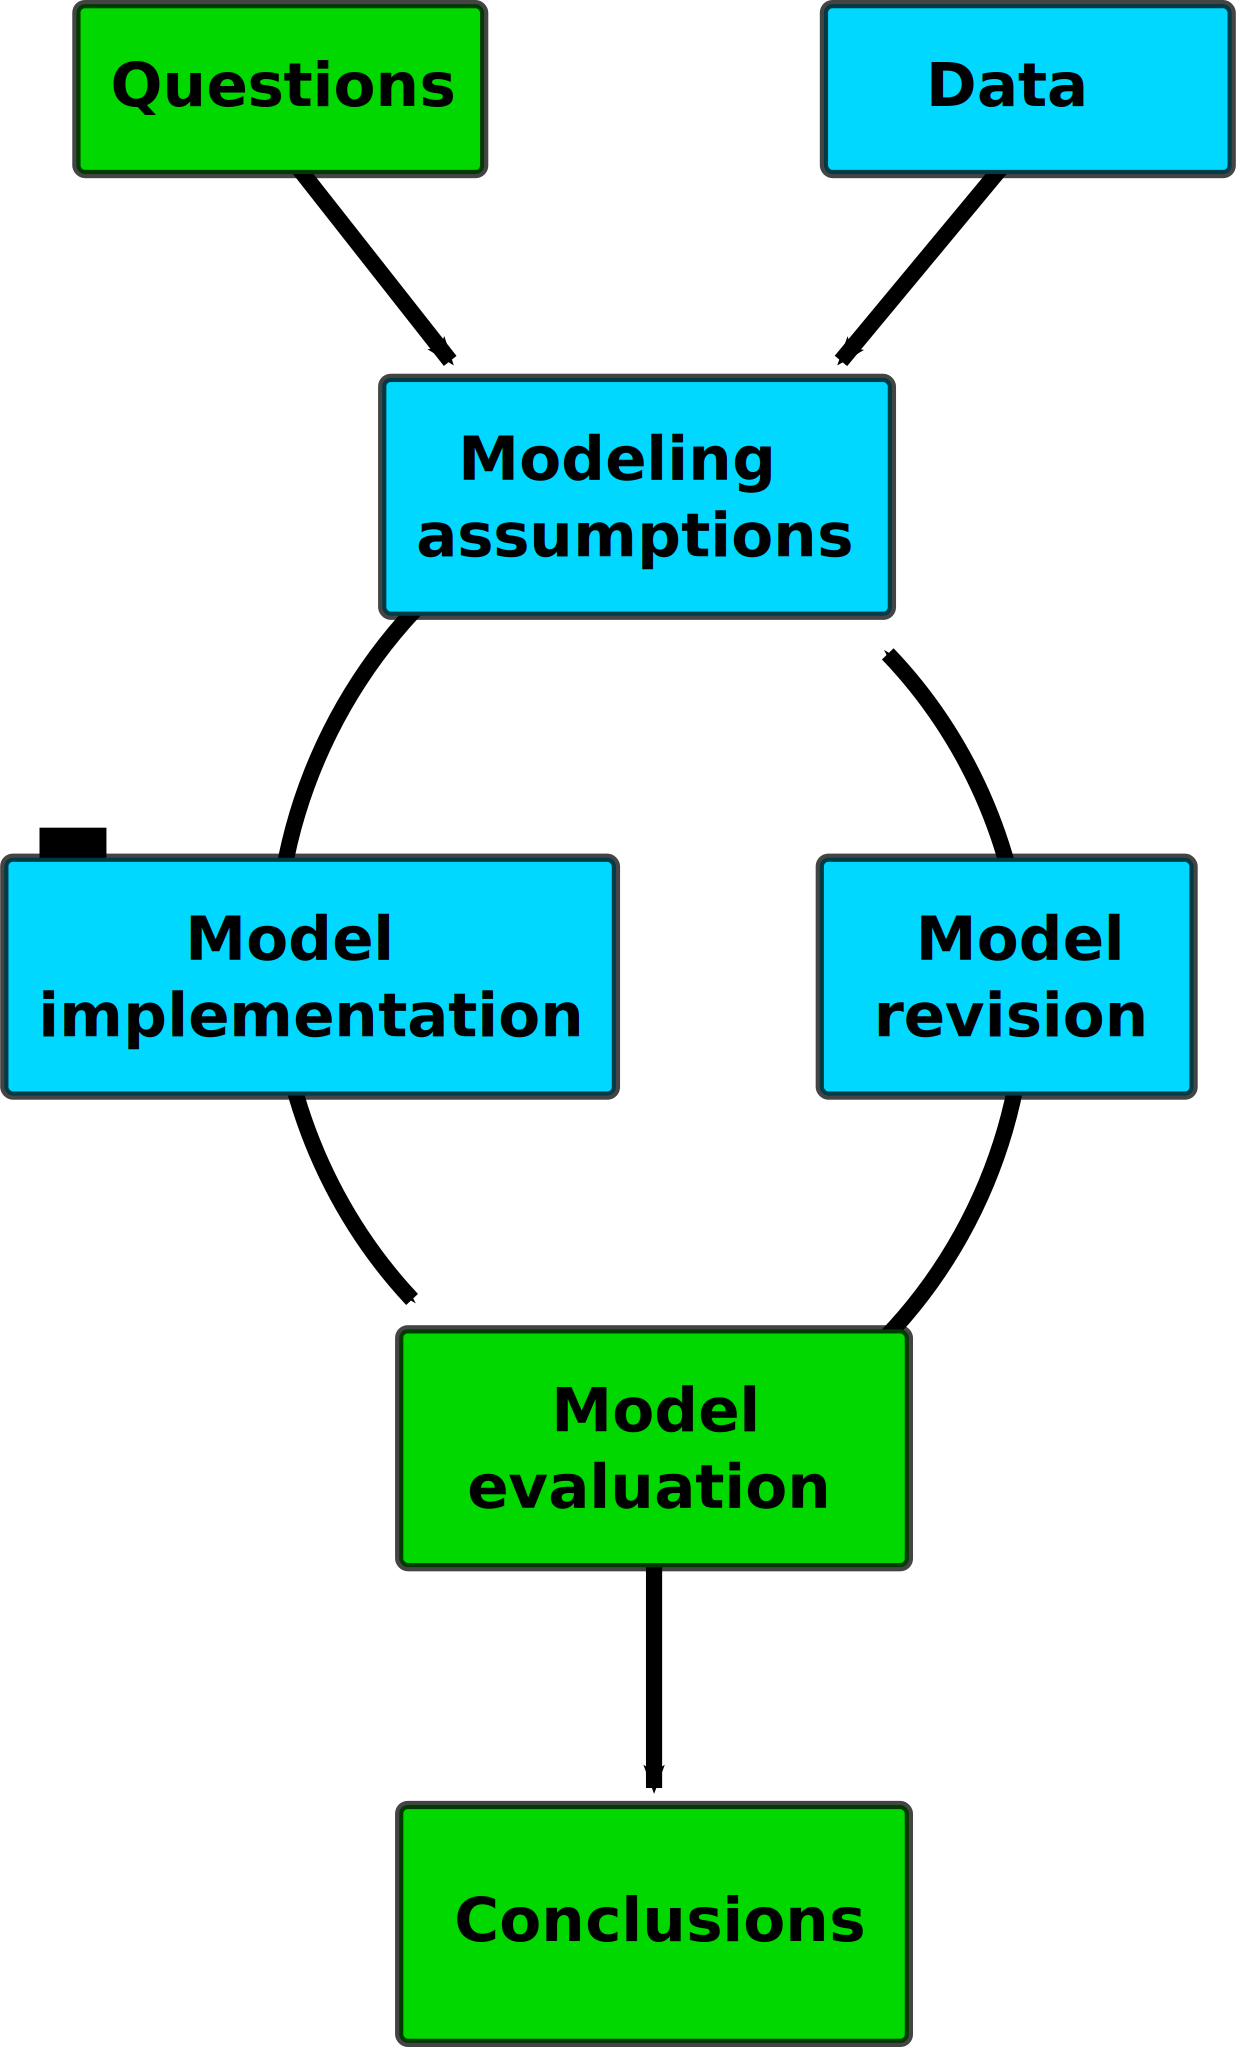
\includegraphics[width=0.4\textwidth]{chapter_introductory_material/figs/model_pipeline.pdf}
  \caption{A data analysis pipeline.  In this work, we discuss
    elements of defining modeling assumptions, model implementation,
    and model revision.  We will focus on applications which use
    text data.}
  \label{figure:data_analysis_pipeline}
\end{figure}

This is then followed by a process of data analysis and exploration,
along with the drawing of conclusions.  This may include visualization
tools such as \cite{chaney:2012}(chaney and blei).

In some cases, the model may be revised.  This revision is ideally
driven by findings in the data analysis step, although our decisions
in the model development step are of course informed by limitations in
the tools available for performing inference and the ease of
subsequent data analysis.
  
  \subsection{Latent-variable models}

  As alluded to above, we will focus on probabilistic models, which
  use both hidden and latent random variables, in stage 2 of the
  pipeline.  Latent variable models have several benefits that appeal
  to us:
  \begin{enumerate}
    \item Flexibility. These models can describe, summarize, and explain
    a wide variety of phenomena in the physical and social sciences.
    \item Embeddability and Interpretability.  Any quantifiable metric in the dataset
      can be encoded as a random variable in a probabilistic model.
      The relationship between metrics can be likewise encoded
      explicity. \label{lvm:matching}
    \item Modularity. Parts of these models can be re-used across
      different models.  This leads to efficient transfer of resources
      and common paradigms.
    \item Existing toolbox of statistical tools. There is a large and
      growing body of literature around how to fit these models.
      Practitioners no longer need to be experts in statistics to
      correctly apply many of these tools.
  \end{enumerate}

  The risk with applying latent-variable models is that the
  credibility and careful deliberation we often associate with
  statistics suggests that an estimated posterior must be
  credible.  This may not be true, particularly when the model is
  poorly embedded into a statistical model, or when it is incorrectly
  interpreted.  Both of these happen when Item~\ref{lvm:matching}
  above is carried out carelessly.

\subsection{Undirected graphical models for summarizing distributional assumptions}
A latent variable model can be fully specified with
\begin{itemize}
  \item A set of latent random variables $X_1, \ldots, X_{M_1}$;
  \item A set of observed random variables $Y_1, \ldots, Y_{M_2}$;
  \item A joint probability distribution $p(X_1, \ldots,
    X_{M_1}, Y_1, \ldots, Y_{M_2})$ indexed by $\theta$.
\end{itemize}
While some practitioners may index this family of probability
distributions with some index set $\{ \theta \}$ with the goal of
learning that index $\hat \theta$ which makes the data most likely, we
will usually focus on a single distribution.  Further, as $p$ is a
probability distribution, it satisfies 
\begin{align*}
  \int_{x_1, \ldots, x_{M_1},
    y_1, \ldots, y_{M_2}} p(X_1, \ldots, X_{M_1}, Y_1, \ldots, Y_{M_2})
  d x_1, \ldots, d x_{M_1}, d y_1, \ldots, d y_{M_2} = 1.
\end{align*}
  
For $p$ to be at all useful, we typically will make distributional
assumptions about it.  We often describe assumptions about
factorization (and conditional independence, which we'll describe
below) using a \emph{graphical model} (sometimes called a Bayesian
network).  A graphical model is a directed, acyclic graph $G = (V, E)$
in which vertices $V=Z_1, \ldots, Z_M$ are random variables and a
\emph{lack} of edges between random variables connotes conditional
independence.

We state this more precisely be defining the ``parents'' function
$\pi_G : V \rightarrow 2^V$, which takes a random variable $Z_m$ to
its parents $\{ Z_i : i \neq m \mbox{ and } (Z_i, Z_m) \in E \}$.  In
the language of graphical models, the distribution of a random
variable $Z_m$ can be specified by its parents. A probability
distribution described by a graphical model $G$ can be factorized as
\begin{align}
  p(Z_1, \ldots, Z_M) = \prod_{i=1, \ldots, M} p_\theta(Z_i | \pi_G(Z_i) ).
\end{align}
Note that there is a many-to-many relationship between graphical
models and probability distributions. Every graphical model may
describe many different distributions (but all such distributions must
be factorizable based on this graphical model).  Likewise, most
distributions can be described by multiple graphical models (but each
distribution must be factorizable based on all of its corresponding
graphical models). Still, the language of graphical models makes it
possible to succinctly describe many joint probability distributions,
and it makes inference with these models much easier to discuss.

A graphical model $G$ is often drawn as a block-and-arrow diagram.  An
additional convention in these diagrams is that boxes, or
\emph{plates}, represent replication (with the number of replications
shown in a corner of the plate). In the graphical model shown in
\myfig{bagofwords_lda_gm} (B), for example, the corresponding factorization is
\begin{align}
  \prod_K p(\beta_k) \times \prod_{d=1,\ldots,D} p(\theta_d | \alpha) \prod_{n=1,\ldots,N_d} p(z_n | \theta_d) p(w_n | z_n, \beta_{z_n})
\end{align}

\begin{figure}
  \begin{center}
    \begin{tabular}{cc}
      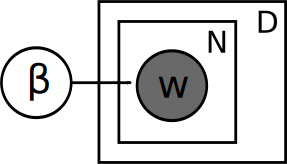
\includegraphics[width=0.2\textwidth]{chapter_introductory_material/figs/bagofwords_gm.pdf} & 
      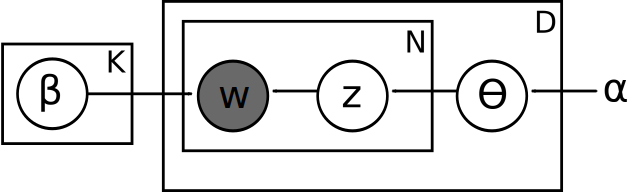
\includegraphics[width=0.4667\textwidth]{chapter_introductory_material/figs/lda_gm.pdf} \\
      Unigram language model & Latent Dirichlet allocation \\
    \end{tabular}
  \end{center}
  \caption{Left: graphical model for a unigram language model.  Documents $1, \ldots, D$ are
    treated as \emph{bags of words}, or collections of words $w_n$.
    Right: graphical model for Latent Dirichlet Allocation.  Circles are random variables, arrows connote dependency, and plates represent replication.  The circles represent observed random variables (words in this case).}
  \label{figure:bagofwords_lda_gm}
\end{figure}

One of the most useful assumptions is conditional independence.  Given
random variables $Z_1, Z_2,$ and $Z_3$, we say that $Z_1$ is
conditionally independent of $Z_2$ given $Z_3$ if $p(Z_1, Z_2 | Z_3) =
p(Z_1 | Z_3) p(Z_2 | Z_3)$ \cite{bishop:2006}.

\subsection{Text as a medium for social science analysis}
  \label{section:text_intro}
  Text data is the low-hanging fruit of most social science research
  questions.  Its ubiquity is due to the ease with which it can be
  both created and digitized.  At the same time, it provides a rich
  source of data: documents, one of the basic units of information in
  text analysis, are an observation in an extremely high-dimensional
  and interpretable space \cite{changrtl:2009}.

  \cite{grimmer:submitted} provides an excellent overview of text
  analysis; we will summarize several methods here.

% \subsection{Latent-variable models of text}
  
  Text data is extremly high-dimensional.  A large collection of
  documents represented by a sequence $\bm w_n$ of words would be
  unweildly for even a human to describe.  A number of tools have been
  developed over the past several decades to simply find the
  \emph{gist} of documents, making it possible to describe collections
  succinctly and efficiently.

  In this work we will use the simplifying assumption that each text
  document can be represented as a vector $\bm w_d \in \mathcal{R}^V$
  of word counts.  This assumption, known as the \emph{bag of words}
  assumption, removes most of the information in a document.  At the
  same time, it allows us to capture the ``gist'' of a document very
  well. One of the simplest bag-of-words models is the unigram
  model. In the unigram model, every word is assumed to come from the
  some multinomial distribution $\beta$ over the vocabulary:
  \[
    p(w_{11}, \ldots, w_{ND}) = p(\beta) \prod_D \prod_{N_d} p(w_{nd} |
  \beta). \]
  We illustrate this model graphically in
  \myfig{bagofwords_lda_gm} (A).  The bag-of-words assumption in
  particular is illustrated by the model's agnostic treatment of the
  order between words: these words are fully exchangeable within each
  document.

\subsubsection{Latent Dirichlet Allocation}
We will capture the gist of documents using the topic model Latent
Dirichlet Allocation \cite{blei:2003}.  Latent Dirichlet allocation
(LDA) posits a set of $K$ \emph{topics} $\beta_1, \ldots, \beta_K$ to
formalize what we mean by the \emph{gist} of a document.  LDA describes each
document $d$ as a mixture $\bm \theta_d$ of themes, where $\sum_K
\theta_{dk} = 1$ and $\theta_{dk} > 0 \forall d,k$.

Formally, we represent this using a generative process of the collection of documents:
\begin{enumerate}
  \item Draw topics $\beta_1, \ldots, \beta_K \sim \mbox{Dir}(\eta)$.
    \item For document $d=1, \ldots, D$:
    \begin{enumerate}
    \item Draw topic mixture $\theta_d \sim \mbox{Dir}(\alpha)$.
    \item For term $n=1, \ldots, N$:
      \begin{enumerate}
      \item Draw topic indicator $z_n \sim \mbox{Mult}(\theta_d)$.
      \item Draw word $w_n \sim \mbox{Mult}(\beta_{z_n})$.
      \end{enumerate}
    \end{enumerate}
\end{enumerate}
Above, the parameter $\alpha > 0$ is a Dirichlet prior, often set to
$1/K$.

The joint distribution of a collection of documents under Latent Dirichlet Allocation is
\begin{align}
  p(\beta_k, \theta, \bm Z, \bm W | \alpha) = 
  \prod_K p(\beta_k)
  \prod_D p(\theta_d) \prod_N p(z_n | \theta_d) p(w_n | z_n, \beta_{z_n}) d\beta d\theta dz,
\end{align}
where $p(\beta_k)$ and $p(\theta_d)$ are understood to be conditioned
on $\eta$ and $\alpha$ respectively (we treat them as hyperparameters
and omit them so they're not confused with random variables).

Before describing how to fit such a model, we show an example of
topics from LDA in \myfig{}.

\begin{figure}
\end{figure}

\subsubsection{Inference}
Of course, we only observe the words $\bm Z$ in a collection of
documents, and we are interested in estimating what the topics $\beta$
and topic mixtures $\theta$ are.  We will generally accomplish this
with posterior inference, in which we aim to estimate the
posterior distribution
\begin{align}
  p(\beta, \theta, \bm Z | \bm W) = \frac{p(W | \beta, \theta, \bm Z) p(\beta, \theta, \bm Z)}{p(\bm W)}. \\
\end{align}

This conditional distribution is impossible to compute because of the
intractable normalizing constant
\begin{align} 
  p(\bm W) = & \prod_K \int_{\beta_k} p(\beta_k)
  \prod_D \int_{\theta_d} p(\theta_d | \alpha) \prod_N \sum_{n=1}^N p(z_n | \theta_d) p(w_n | z_n, \beta_{z_n}) d\beta d\theta dz.
\end{align}
\mysec{variational_inference} provides details on how to get around
this by approximating the posterior above.

We will use topic models like LDA for several purposes in later
sections.

%\subsubsection{Unigram models}
%  One of the simplest bag-of-word language models is a unigram model

%\subsubsection{Regression}
% One of these applications is prediction. In the simplest of these   In text regressionWe will see in later sections that topic models can be used for
% prediction by using Text regression is a

\subsection{Ideal point models and matrix factorization}

One of the most common primitives in latent-variable models is matrix
factorization \cite{salakhutdinov:2008a}. We will discuss a specific
application of matrix factorization called item response theory (IRT),
which has been used for decades in political science
\cite{clinton:2004,martin:2002,poole:1991,enelow:1984,albert:1992}.

In IRT, we have two types of objects, and we would like to make
predictions about pairs of them.  Each of these objects -- suppose
that they are lawmakers and bills, to be concrete -- is represented by
real-valued random variables: lawmaker $u \in \{ u=1, \ldots, U \}$
has a latent value $X_u \in \mathbb{R}$, and each bill $d \in \{ 1,
\ldots, D \}$ has two latent values $A_d,B_d \in \mathbb{R}$.  We make
predictions about pairs of them by introducting the likelihood
function $p(V_{ud} | X_u, A_d, B_d) = \sigma( x_u a_d + b_d )$, where
$\sigma(s) = \frac{\exp(s)}{ 1 + \exp(s) }$.

More formally, we can say that the matrix $\{V\}_{ud}$ of boolean outcomes (for example, votes) is represented with the matrix product
\begin{align}
  \hat \sigma \left( \left[ \begin{array}{cc}
    x_1 & 1 \\
    \vdots & \vdots \\
    x_U & 1 \\
  \end{array}
  \right]
  \left[
    \begin{array}{ccc}
      a_1 & \cdots & a_D \\
      b_1 & \cdots & b_D \\
    \end{array}
    \right]^T 
  \right),
\end{align}
where the matrix operator $\hat \sigma(\cdot)$ produces a matrix in
which the scalar logistic function $\sigma(s) = \frac{\exp(s)}{1 +
  \exp(s)}$ is applied to each element of its argument.

\begin{figure}
  \begin{center}
  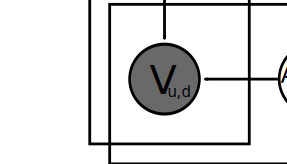
\includegraphics[width=0.3\textwidth]{chapter_introductory_material/figs/irt_gm.pdf}
  \end{center}
  \caption{Probabilistic matrix factorization.  We observe
    interactions $V_{ud}$ between users represented by $X_u$ and items
    represented by $A_d, B_d$.}
  \label{figure:irt_gm}
\end{figure}

A wide variety of researchers have used formulations like this for
applications such as recommendation and representing the votes of
lawmakers \citet{wang:2011,salakhutdinov:2008a,poole:1985,poole:1991,clinton:2004}. In later chapters, we will use it for models of legislative voting.

% Recent 
%   - relevant sources
%   - mathematical foundation
%   - examples
%   - hinge loss
%   - inference (stochastic)

\subsection{Hidden Markov Models and Kalman Filters}
We now turn briefly to abstractions for time-series data.  Consider a
typical scenario: a sequence of observations $Y_1, \ldots, Y_T$ are
observed at times $t=1, \ldots, t=T$.  In a \emph{hidden Markov model}
(HMM), we assume that these observations can be explained by a hidden set of states $X_1, \ldots, X_T$.  The model factorizes as
\begin{align}
  p(Y_1, \ldots, Y_T, X_1, \ldots, X_T) = p(X_1) p(Y_1 | X_1) \times \prod_{t=2, \ldots, T} p(X_t | X_{t-1}) p(Y_t | X_t)
\end{align}
(see \myfig{hmm_gm} for the graphical model).  Often the transition
distribution $p(X_t | X_{t-1})$ is independent of $t$ (the chain in
this case is called \emph{time-homogenous}.  A wide variety of
problems can be modeled accurately with a well-selected homogeneous
HMM.  Importantly, inference in these models is very efficient because
the set of conditional independencies yields a tree: inference can
usually be reduced to an application of a forward-backward algorithm.
One of the most famous examples of a hidden Markov model is the Kalman
filter, which assumes linear (or quadratic) transitions between the
states $X$ and Gaussian noise: $p(Y_t | X_t) \propto \mathcal{N}(X_t,
\sigma^2)$ for some variance $\sigma^2$.
\begin{figure}
  \begin{center}
  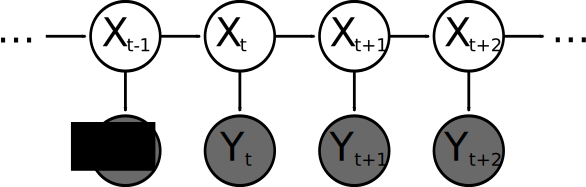
\includegraphics[width=0.6\textwidth]{chapter_introductory_material/figs/hmm_gm.pdf}
  \end{center}
  \caption{A hidden Markov model.  Observations $Y_1, \ldots, Y_T$ are observed at discrete times $t=1, \ldots, T$, and are conditionally independent given the hidden states $X_1, \ldots, X_T$.}
  \label{figure:bagofwords_lda_gm}
\end{figure}

It is worth pointing out that many language models \emph{do}
incorporate the order of words.  Part-of-speech taggers, for example,
often use hidden Markov model assumptions, treating words as observed
and part-of-speech as tags.  While these assumptions are useful for
some applications, we will use the bag-of-words assumption described
in \mysec{text_intro}.

% TODO(sgerrish): cite Kalman.

\section{Posterior inference and model evaluation}
One of the most fundamental problems in statistical machine learning
is that of estimating the values of latent random variables $X$ in a
statistical model, given observed random variables $Y$.  In this work, we will
focus on estimates of the posterior distribution $p(x | y) =
\frac{p(x, y)}{p(y)}$.

\subsection{MAP estimation}
One of the simplest estimates the value of a random variable is the \emph{maximum-a-posteriori} (MAP) estimate.  The MAP estimate $\hat X$ is defined to be the most-likely value of the random variable:
\begin{align}
  \hat X = \arg \max_x p(X=x | Y) = \arg \max_x \frac{p(X=x | Y) p(Y)}{p(Y)} = \arg_x \max p(X=x, Y).
\end{align}

The MAP estimate can typically found by performing gradient or
coordinate ascent on $p(X, Y)$ with respect to $X$ (this is because
the normalizer $p(Y)$ is not a function of $X$).  Because MAP
estimates can be fast to estimate, they can shorten the development
loop described in \mysec{pipeline}. The MAP provides a point estimate
which is often a good summary of the posterior distribution.

\subsection{MCMC}

% Markov Chain Monte-Carlo (MCMC) methods provide a method for drawing
% samples $x_m$ from a posterior distribution $p(X | Y)$.

We briefly review the key components of Markov Chain Monte Carlo
(MCMC) estimation.  We will not go into detail about MCMC in this work except to
draw a contrast with variational methods (which are introduced in the
next section), and readers unfamiliar with MCMC can refer to a
standard text such as Bishop et al. \cite{bishop:2006}.

% Markov Chain Monte-Carlo methods provide non-independent samples from
% a posterior.  These samples are unbiased, and, when the number of
% samples is large, they can be used to reliably estimate arbitrary
% statistics of a posterior distribution (such as marginal mean and
% variance).

MCMC methods are often used to inspect a posterior distribution $p(x |
y)$.  The input to an MCMC sampler is typically an unnormalized
probability density $\tilde p(x, y) \propto p(x | y)$ \footnote{For
  numerical and algebraic convenience, $\tilde p(x, y)$ is often
  specified by $\log \tilde p(x, y)$.}  Given $\tilde p(x, y)$, an
MCMC sampler produces a collection of samples from $p(x | y)$.  These
samples are often used to summarize statistics such as marginal means
and variances of $p(x | y)$.  They are unbiased and, given enough
time, will accurately represent $p(x | y)$.

MCMC methods are used widely, and they have well-known limitations.
One of these limitations is runtime: while one may need $N$ \emph{iid}
samples from a distribution $p(x | y)$ to estimate its mean and
variance, he typically needs many more MCMC samples to estimate these
statistics.  A poorly-chosen proposal distribution can affect runtime,
as a Markov chain needs more samples to converge. MCMC algorithms can
also suffer from memory bottlenecks, as samples are stored and
convergence is measured.

Even when memory is not a bottleneck, the
practitioner is often interested in only the marginals of the
posterior (as with most mixture-of-Gaussian applications); a large
number of discarded samples indicates that there is an inefficiency in
the inference pipeline.

\subsection{Variational inference}
\label{section:variational_inference}

Variational methods address some of the shortcomings of MCMC by
providing a fast, deterministic alternative to MCMC
\cite{jordan:2003,jordan:1999}.  We review the key ideas here and will
use use these methods as we develop models in later chapters.

Variational methods posit a simplified
family $\mathcal{F}$ of distributions and select the member $q_\theta
\in \mathcal{F}$ of this family that is closest in KL-divergence to
the true posterior $p(x | y)$:
\begin{align}
  \arg \min_{q_\theta \in \mathcal{F}} \mbox{KL}(q_\theta || p) = \arg \min_{q_\theta \in \mathcal{F}} \int_x q_\theta(x) \log \frac{q_\theta(x)}{p(x | y)} dx.
  \label{equation:variational_objective}
\end{align}
Finding the optimal variational distribution $q_\theta \in
\mathcal{F}$ is equivalent to optimizing an ``evidence lower bound''
($\mbox{Elbo}_\theta$) on the data likelihood
\begin{eqnarray}
  \log p(y) \ge \expectq{\log p(x, y) - \log q_\theta(x)}
  =: \mbox{Elbo}_\theta,
  \label{equation:traditional_variational_objective}
\end{eqnarray}
where the slack of the bound is equal to the KL divergence from
Equation~\ref{equation:variational_objective}.

The family $\mathcal{F}$ is chosen by the practitioner to make the
resulting algorithm tractable and to capture the parameters of
interest. A common assumption is that the posterior is
fully-factorized into simple marginal distributions; such an
assumption is known as \emph{naive mean-field variational inference}.

For example, a multivariate posterior $p(x | Y), x \in \mathcal{R}^D$
might be represented by the product $q(x) = \prod_D \mathcal{N}(\mu_d,
\sigma_d^2)$ of $D$ Gaussian distributions. and a Dirichlet
distribution might represent a multinomial random variable
\cite{bishop:2006}.  In the case of Latent Dirichlet Allocation, for
example, \citet{blei:2003} assume that the indicators $z_n$ can be
described by a fully-factorized product of multinomial distributions,
and they assume that the topics $\beta$ and mixture proportions
$\theta$ can be represented by a fully-factorized product of Dirichlet
distributions.

Once a family is selected, the bound in
Equation~\ref{equation:traditional_variational_objective} is evaluated
symbolically, as a practitioner fully expands $\expectq{ \log p(x, y)
  - \log q_\theta(x)}$ and (usually) its gradient. This bound may
itself be bounded or approximated with a Taylor approximation such as
the delta method \cite{bickel:2007,braun:2007}. These simplifying
assumptions -- an approximate, fully factorized posterior with further
simplifying bounds -- make it possible to express the lower bound in
terms of the variational parameters $\theta$.  This is followed by
coordinate or gradient ascent.

The role of variational inference in statistical machine learning will
become more clear as we develop several algorithms using these methods
over the next two chapters.  Later we will also consider an
alternative method for performing variational inference.  This
alternative method will remove the onus of deriving new variational
updates from the practitioner, making it easy to perform rapid model
development on simple models.

% \subsection{Stochastic optimization}
%   - examples

% \subsection{Posterior Predictive Checks}
%   - examples
\subsection{Model evaluation}
As we progress through the pipeline described in \mysec{pipeline}, it
is important to evaluate the model.  The quality of a model depends on
the practitioner's goals, so evaluation methods differ greatly.
However, several standard metrics exist.

\subsubsection{Likelihood of heldout observations $Y_1, \ldots, Y_{N_{\mbox{heldout}}}$}
One of the most common metrics of a model is its ability to model
unseen observations $Y_{\mbox{heldout},1}, \ldots,
Y_{\mbox{heldout},N_{\mbox{heldout}}}$.  One of the most frequently
used metrics for this is the log-likelihood $\log
p(Y_{\mbox{heldout},1}, \ldots, Y_{\mbox{heldout},N_{\mbox{heldout}}} |
  Y_1, \ldots, Y_{N_{\mbox{obs}}}, X )$ of these observations. When
  these observations are conditionally independent given the observed
  data (nearly always the case), the log-likelihood can be
  written $\sum_{n=1}^N \log p(Y_{\mbox{heldout},n} | Y_1{\mbox{observed}},
  X)$.\footnote{This log-likelihood is frequently exponentiated to
    yield perplexity.}

\subsubsection{Likelihood of training data $Y_1, \ldots, Y_{N_{\mbox{obs}}}$}
For completeness, we note that an even simpler metric of a model is its ability to model training data
$Y_{\mbox{obs},1}, \ldots, Y_{\mbox{obs},N_{\mbox{obs}}}$.
One of the most frequently used metrics for this is the log-likelihood
$\log p(Y_{\mbox{obs},1}, \ldots,
Y_{\mbox{obs},N_{\mbox{obs}}} | Y_1, \ldots,
Y_{N_{\mbox{obs}}}, X )$ of these observations. When these
observations are conditionally independent given the observed data
(nearly always the case), the log-likelihood can be written
$\sum_{n=1}^N \log p(Y_{\mbox{heldout},n} | Y_1{\mbox{obs}}, X)$.
The downfall of this metric is of course that it does not measure whether a model is overfit.

% \subsubsection{Predictive accuracy}
% When a model is created for the purpose of making predictions, heldout
% log-likelihood is often not an appropriate measure of that model's
% performance.  To be concreate, consider a model developed to predict
% the maximum

% \subsubsection{Relationship with external observations}
% Sometimes a model A final metric that we will consider is a model's
% relationship to outside data -- data which was not directly
% incorporated into the model.

% In a model we will develop later, we are operating in a
% vacuum: This can be useful when, for example, the model
